\documentclass[12pt,a4paper]{report}
\usepackage[utf8]{inputenc}
\usepackage[spanish]{babel}
\usepackage{graphicx}
\usepackage{float}
\usepackage{geometry}
\usepackage{fancyhdr}
\usepackage{titlesec}
\usepackage{xcolor}
\usepackage{hyperref}
\usepackage{enumitem}
\usepackage{tcolorbox}
\usepackage{tikz}

% Configuración de página
\geometry{left=2.5cm, right=2.5cm, bottom=2.5cm, top=1.5cm}
\pagestyle{fancy}
\fancyhf{}
\fancyhead[L]{\leftmark}
\fancyhead[R]{\thepage}
\renewcommand{\headrulewidth}{0.4pt}

% Colores personalizados
\definecolor{primary}{RGB}{33, 150, 243}
\definecolor{secondary}{RGB}{96, 125, 139}
\definecolor{accent}{RGB}{255, 193, 7}
\definecolor{darkgray}{RGB}{66, 66, 66}

% Configuración de hyperlinks
\hypersetup{
    colorlinks=true,
    linkcolor=primary,
    filecolor=magenta,      
    urlcolor=primary,
    pdftitle={Guía de Pantallas - Aplicación de Despachos},
    pdfauthor={Equipo de Desarrollo},
    pdfsubject={Documentación de Usuario}
}

% Formato de títulos
\titleformat{\chapter}{\huge\bfseries\color{primary}}{\thechapter.}{1em}{}
\titleformat{\section}{\Large\bfseries\color{secondary}}{\thesection}{1em}{}
\titleformat{\subsection}{\large\bfseries\color{darkgray}}{\thesubsection}{1em}{}

% Entorno para pantallas
\newtcolorbox{pantallabox}{
    colback=blue!5!white,
    colframe=primary,
    boxrule=2pt,
    rounded corners,
    left=10pt,
    right=10pt,
    top=10pt,
    bottom=10pt
}

% Entorno para características
\newtcolorbox{caracteristicabox}{
    colback=green!5!white,
    colframe=green!50!black,
    boxrule=1pt,
    rounded corners,
    left=8pt,
    right=8pt,
    top=5pt,
    bottom=8pt
}

\begin{document}

% Página de título
\begin{titlepage}
    \centering
    \vspace*{2cm}
    
    {\Huge\bfseries\color{primary} GUÍA DE PANTALLAS}\\[0.5cm]
    {\LARGE\color{secondary} Aplicación de Gestión de Despachos}\\[2cm]
    
    % Aquí puedes agregar el logo de la empresa
    % \includegraphics[width=0.3\textwidth]{logo.png}\\[2cm]
    
    {\Large Manual de Usuario}\\[1cm]
    {\large Versión 1.4.2}\\[2cm]
    
    \vfill
    
    {\large \today}
\end{titlepage}

% Tabla de contenidos
\tableofcontents
\newpage

% Introducción
\chapter{Introducción}

\section{Propósito del Documento}
Esta guía presenta las diferentes pantallas de la aplicación de gestión de despachos, detallando su funcionalidad y uso para facilitar la experiencia del usuario.

\section{Alcance}
El documento cubre todas las pantallas principales de la aplicación, incluyendo navegación, características principales y flujos de trabajo.

\section{Audiencia}
Este documento está dirigido a usuarios finales, personal de soporte técnico y administradores del sistema.

% Pantalla Principal
\chapter{Pantalla Principal}

\begin{pantallabox}
\textbf{Pantalla:} Inicio/Menú Principal \\
\textbf{Archivo:} \texttt{sp\_main\_home\_screen.dart}
\end{pantallabox}

\section{Descripción General}
La pantalla principal sirve como punto de entrada a todas las funcionalidades de la aplicación.

\section{Imagen de la Pantalla}
% Espacio para imagen
\begin{figure}[H]
    \centering
    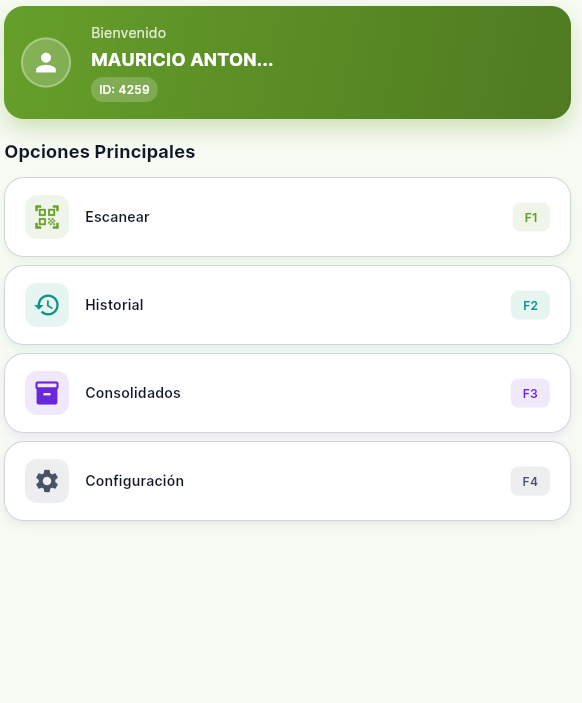
\includegraphics[width=0.6\textwidth]{pantallas/dashbord.png}    
    \caption{Pantalla Principal - Menú}
    \label{fig:main_home}
\end{figure}

\section{Características Principales}
\begin{caracteristicabox}
\begin{itemize}[leftmargin=*]
    \item Acceso rápido a módulos principales.
    \item 1- Escaneo de codigo de barra.
    \item 2- Historial de rutas escaneadas (Activos, Finalizados, Todos).
    \item 3- Consolidado de día.
    \item 4- Configuración.
\end{itemize}
\end{caracteristicabox}

% Gestión de Rutas
\chapter{Gestión de Rutas y Consolidado}

\section{Ruta}

\begin{pantallabox}
\textbf{Pantalla:} Escaneo de Códigos de Barras \\
\end{pantallabox}

\subsection{Descripción}
Permite escaner hojas de despacho generadas y asignarlas al dispositivo por medio del usuario.
\subsection{Imagen de la Pantalla}
\begin{figure}[H]
    \centering
      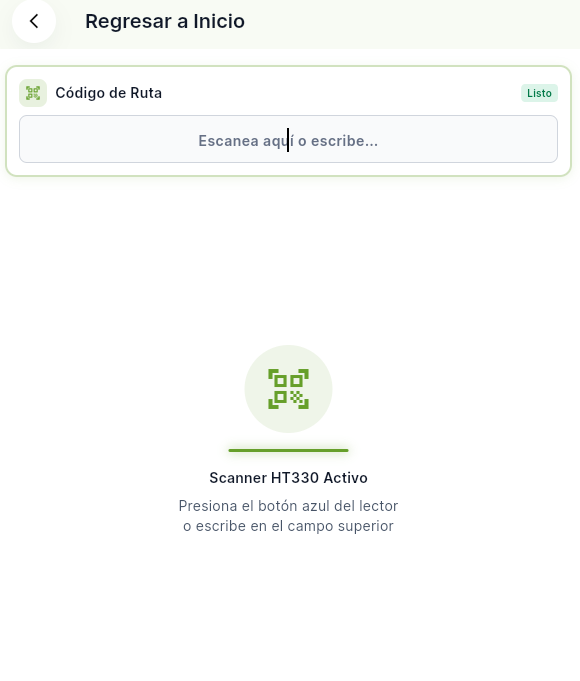
\includegraphics[width=0.6\textwidth]{pantallas/pantallaEscaneo.png} 
    \caption{Pantalla de Escaneo de Código de Barras}
    \label{fig:scan_barcode}
\end{figure}

\subsection{Funcionalidades}
\begin{caracteristicabox}
\begin{itemize}[leftmargin=*]
    \item Escaneo automático de códigos y de forma manual (Presional bottom Azul de aparato)
    \item 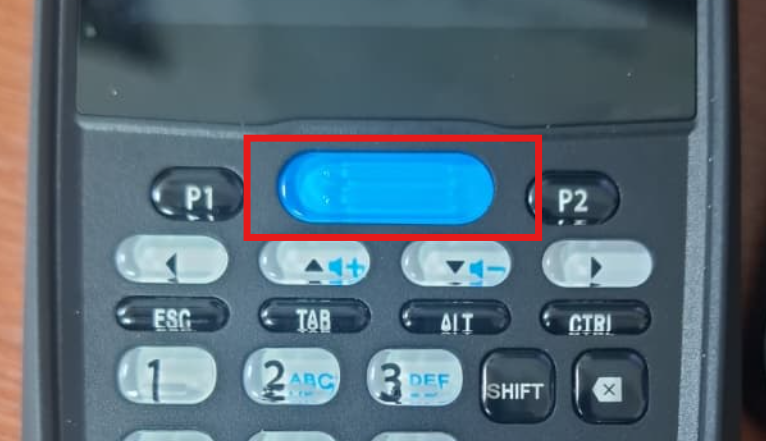
\includegraphics[width=0.2\textwidth]{pantallas/btonAzul.png}
\end{itemize}
\end{caracteristicabox}

\begin{itemize}[leftmargin=*]
    \item Detalle de Escaneo : 
    \item 1- Cantidad de productos
    \item 2- Cajas totales
    \item 3- Unidades totales
    \item 4- Kg. totales
    \item 5- Bodega principal
\end{itemize}
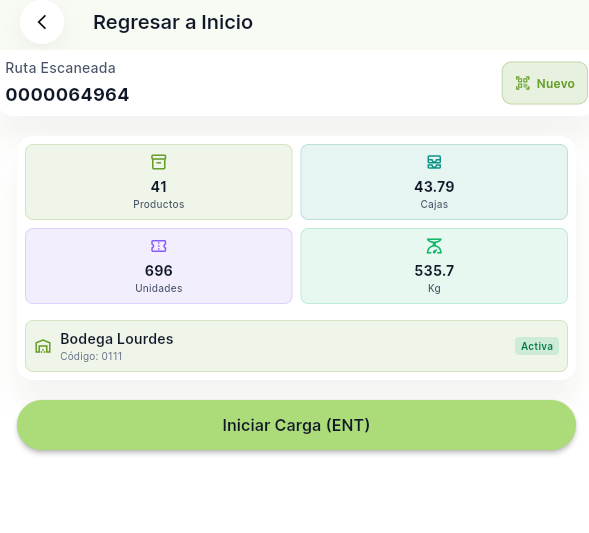
\includegraphics[width=0.6\textwidth]{pantallas/detalleEscaneo.png}

\subsection{Detalle ruta escaneada}
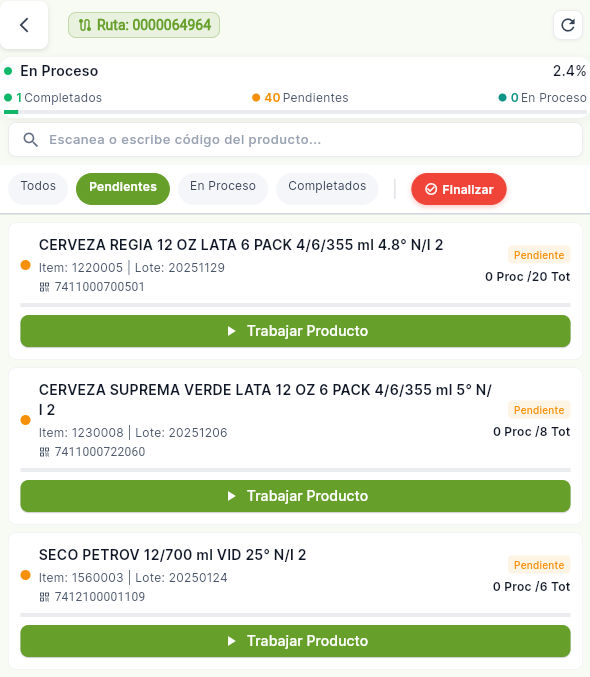
\includegraphics[width=0.6\textwidth]{pantallas/detalleRutaElaborada.png}

\subsection{Botón Trabajar Producto}

\begin{figure}[H]
    \centering
    \begin{minipage}{1.0\textwidth}
        \centering
        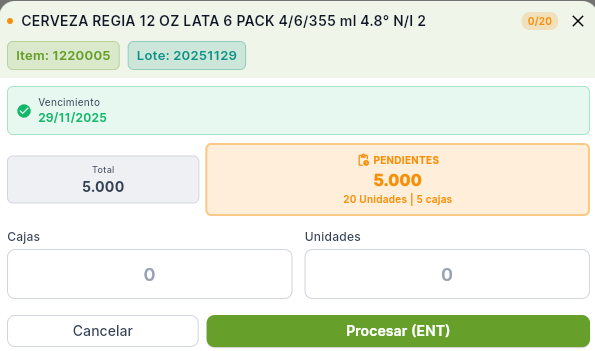
\includegraphics[width=\textwidth]{pantallas/menuProcesarProducto.png}
    \end{minipage}
    \hfill
    \begin{minipage}{1.0\textwidth}
        \textbf{Detalle de Elementos:}
        \begin{enumerate}
            \item \textbf Nombre del producto
            \item \textbf Información del ID Producto y Lote
            \item \textbf Fecha Vencimiento (Sí aplica)
            \item \textbf Total producto
            \item \textbf PENDIENTE = Cantidad (Cajas.0 Unidades) 
            \item \textbf{Campo Cajas}: Ingresa solo Cajas completas
            \item \textbf{Campo Unidades}: Ingresa Unidades totales o parcial
            \item \textbf{Botón Confirmar}: Procesar producto
        \end{enumerate}
    \end{minipage}
\end{figure}

\begin{caracteristicabox}
  Generamos detalle de ruta, donde se permite escanear codigo de producto. 
  \begin{itemize}[leftmargin=*]
    \item Estados = Todos, Pendientes, En Proceso, Completos
    \item Boton de Finalizar: nos permite finalizar ruta completo o con productos incompletos siempre y cuando exista un motivo (Ejemplo : producto dañado o en no existencia)
    \item 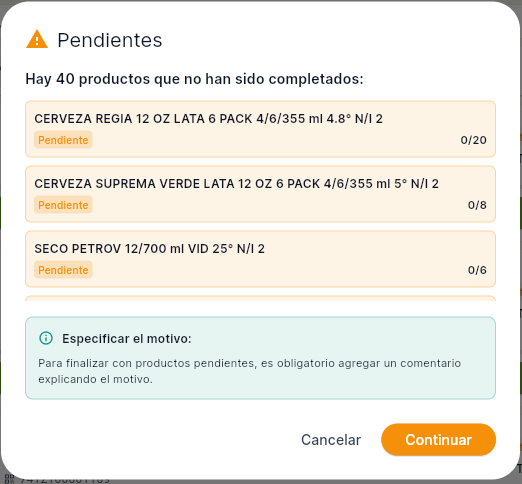
\includegraphics[width=0.3\textwidth]{pantallas/pendientesP.png} 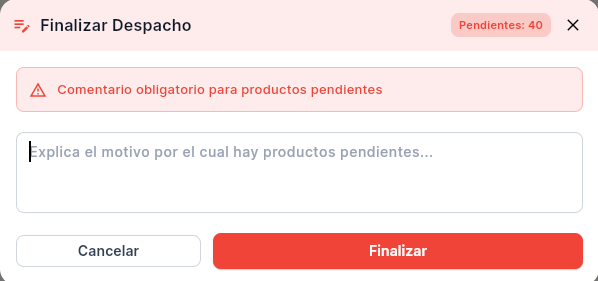
\includegraphics[width=0.6\textwidth]{pantallas/motivoPendiete.png}
\end{itemize}
\end{caracteristicabox}


\section{Pantalla Historial despacho}

\begin{pantallabox}
\textbf{Pantalla:} Lista rutas escaneados por usuario \\
\end{pantallabox}
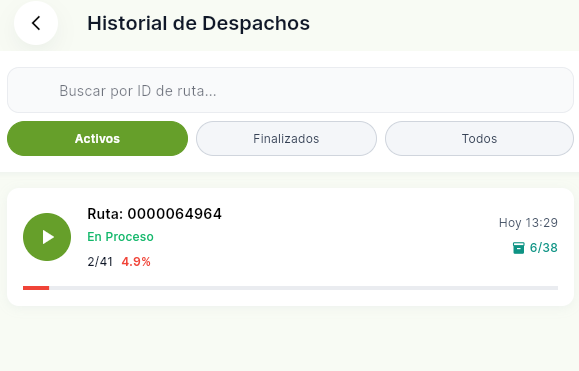
\includegraphics[width=\textwidth]{pantallas/historialDespacho.png}



\section{Pantallas Consolidado}

\begin{pantallabox}
\textbf{Pantalla:} Pantalla de consolidado \\
\end{pantallabox}

\subsection{Imagen de la Pantalla}
\begin{figure}[H]
    \centering
    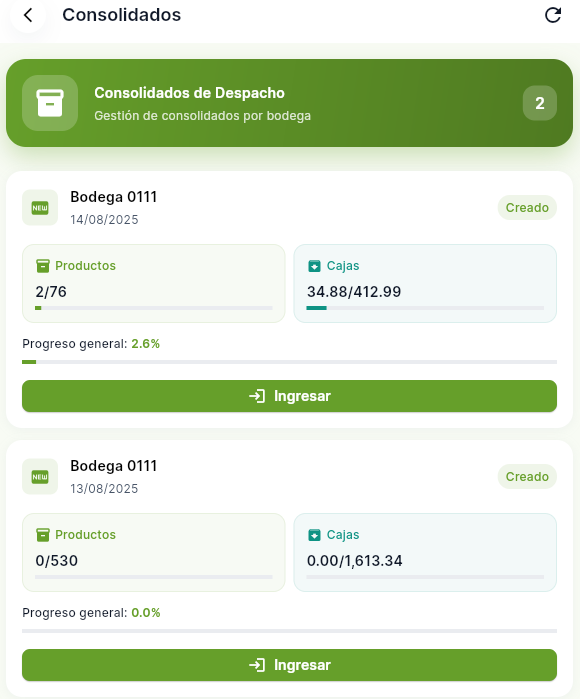
\includegraphics[width=\textwidth]{pantallas/consoldiados.png}
    \caption{Historial de consolidados por Bodega}
    \label{fig:consolidado_detalle}
\end{figure}

\subsection{Descripción}
Muestra consolidados generados en el dia por bodega.

% Configuración y Perfil
\chapter{Configuración y Perfil}

\section{Pantalla de Perfil}

\begin{pantallabox}
\textbf{Pantalla:} Perfil de Usuario \\
\end{pantallabox}

\subsection{Descripción}
Permite al usuario ver su información personal , cerrar sesión  y acceder al repositorio de actualizacion de la Aplicación

\subsection{Imagen de la Pantalla}
\begin{figure}[H]
    \centering
     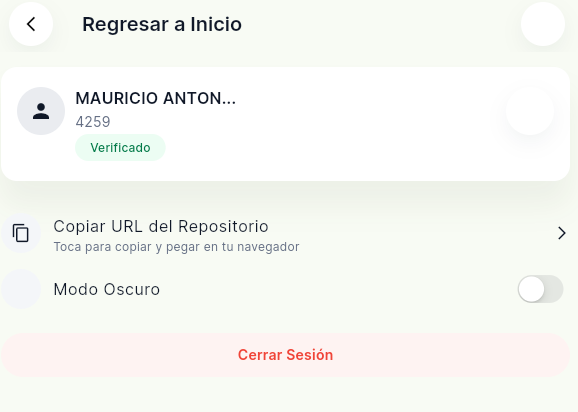
\includegraphics[width=\textwidth]{pantallas/configuracion.png}
    \caption{Pantalla de Perfil de Usuario}
    \label{fig:profile}
\end{figure}

\subsection{Funcionalidades}
\begin{caracteristicabox}
\begin{itemize}[leftmargin=*]
    \item Información del usuario
    \item Acceso al repositorio del proyecto
    \item Opciones de cierre de sesión
    \item Enlaces útiles
\end{itemize}
\end{caracteristicabox}

\chapter{Flujos de Trabajo}

\section{Proceso de Despacho Completo}
\begin{enumerate}
    \item Acceso desde pantalla principal
    \item Selección de ruta/consolidado
    \item Escaneo de productos
    \item Validación y confirmación
    \item Finalización del despacho
    \item Registro en historial
\end{enumerate}

\section{Navegación entre Pantallas}
El sistema utiliza un patrón de navegación jerárquico con opciones de retorno a la pantalla principal desde cualquier punto de la aplicación.

\end{document}